% !TeX root = ../main.tex
\section{Introduction}
\label{sec:introduction}
%
Semiconductor lasers are fundamental components in modern photonic technologies.
Most importantly, their emission wavelengths align with those used in optical communication networks, making them valuable light sources. 
In addition, they are orders of magnitude smaller than typical helium–neon lasers, with coherence lengths of only a few millimetres compared to many metres, which enables widespread practical applications \cite{heiskanen2018photobiomodulation}.
Semiconductor lasers are not only smaller than conventional gas lasers, but also exhibit much higher output coupling, with approximately 70\% of the light intensity escaping them compared to 1-5\% for gas lasers \cite{vantartwijk1995semiconductor}.
However, this openness makes semiconductor lasers more susceptible to external disturbances, leading to a strong response to incident signals.
Although undesirable in some practical applications, this sensitivity has made semiconductor lasers a central platform for investigating nonlinear dynamics induced by external optical feedback.
The influence of external light on laser operation has been extensively investigated since the 1970s, with particular focus on conventional optical feedback (COF) (typically achieved by reflecting output laser light back into the laser cavity using a mirror) as well as on optical injection of laser light from another laser \cite{weiss1991dynamics}.
Feedback and injection mechanisms have important practical implications: for example, the former arises in the operation of CD players, while the latter is central to laser amplification systems.
Beyond their direct historical significance, semiconductor lasers with feedback underpin key technologies in modern photonics. 
Feedback control is exploited to stabilize frequency and linewidth in coherent optical communication \cite{tkach2003regimes}, to enhance sensitivity in precision sensing and metrology, and to enable secure chaos-based encryption schemes \cite{uchida2008fast}. 
At the same time, semiconductor lasers with feedback provide a prototypical and experimentally accessible example of delay differential equations (DDEs), serving as a platform to study nonlinear dynamics with relevance extending to control theory \cite{stepan1989retarded}, electronics, and biological systems \cite{mackey1977oscillation}.
%
%
\subsection*{Lang-Kobayashi equations}
A major breakthrough in understanding the dynamics of semiconductor lasers with external feedback came in 1980 with the seminal work of Lang and Kobayashi, who introduced what are now known as the Lang–Kobayashi (LK) rate equations. 
These equations provide a description of the coupled carrier and optical field dynamics of a semiconductor laser subject to COF from a distant mirror \cite{lang1980external}.
These equations describe the coupled dynamics of the complex electric field $E = E_x + iE_y$ and the carrier inversion $N$ in a semiconductor laser subject to COF from a distant mirror \cite{lang1980external}.
A nondimensionalized form of these equations, highlighting the key parameters governing the system dynamics, is given by \cite{heil2003delay}
%
\begin{equation}
\label{eq:LK}
    \begin{aligned}
        \frac{d E}{d t} & =(1+i \a) N(t) E(t)+\eta F(t) \\
        T \frac{d N}{d t} & =P-N(t)-(1+2 N(t))|E(t)|^2
    \end{aligned}
\end{equation}
%
where the feedback term is given by $F(t) = e^{-i \w_0 \tau} E(t-\tau)$. 
These key parameters can be separated into intrinsic laser parameters and external cavity (EC) parameters. 
The laser, emitting at a single frequency $\w_0$, is characterised by the pump current $P$, the linewidth enhancement factor $\a$, and the ratio of photon and electron decay times $T = \tau_e/\tau_p$. 
The external cavity (EC), which in this context is implemented as an optical fibre with refractive index $n_{eff}$, is characterised by the round-trip delay time $\tau = 2L_\text{EC}/n_{eff} c$, the feedback power level (defined as the ratio of power reflected from the external mirror to that from the diode mirror) $\eta$, and the feedback phase $C_p = \w_0 \tau$, corresponding to the number of optical wavelengths in the EC.
It is noted that these equations are formulated with reference to the centre frequency of the laser, with $\wZ = 0$ at the operating frequency, which implies $C_p = 0$ in the first instance. 
The application of these equations requires a single-mode laser subject to weak feedback (up to a few percent of the emitted light) from a long EC, typically ranging from centimetres to metres in length. 
These assumptions impose several important limitations on the LK model, which can be grouped into restrictions on the laser operating frequency, the cavity, and the feedback strength.
As the LK equations assume single-mode operation, they do not capture mode competition or spectral dynamics; for approaches to the analysis of multimode lasers, see \cite{yacomotti2004dynamics} and references therein.
A long EC justifies treating the feedback phase $C_p$ as an independent parameter from the delay $\tau$, since a $2\pi$ phase shift corresponds to only a half-wavelength change (about one micron) in the cavity length, which is negligible at these scales \cite{green2006mode}. 
In practice, varying $C_p$ over a full $2\pi$ is achieved by shifting the mirror position using a piezoelectric transducer \cite{heil2003delay} for example, or by changing thermal properties of the cavity itself, introducing a slight variation to the fibre's refractive index and thus effective cavity length \cite{skenderas2021feedback}.
The weak-feedback condition further ensures that multiple EC reflections between the laser facet and the external mirror can be neglected; if this condition is not satisfied, the feedback $F(t)$ takes a more complex form \cite{vantartwijk1995semiconductor}.
%
\begin{equation}
\label{eq:multiple_EC}
    F(t) = \frac{R_2^{\;2} - 1}{R_2^{\;2}} \sum_{n=1}^\infty (-R_2 R)^n e^{-i n C_p} E(t-n \tau)
\end{equation}
%
where $R$ is the reflectivity of the external mirror and $R_2$ is the reflectivity of the laser facet.
%
\par
%
The LK equations successfully capture the rich dynamical behaviours of semiconductor lasers under weak external feedback, including steady-state, periodic, quasi-periodic, and chaotic emission, as well as complex behaviours such as regular pulse packages (RPPs), coherence collapse (CC), and low-frequency fluctuations (LFFs) \cite{heil1998coexistence}.
The delay $E(t-\tau)$ present in the feedback term $F(t)$ makes the LK equations DDEs with phase space in the infinite-dimensional Banach space $C([-\tau,0],\mathbb{C}\times\mathbb{R})$, consisting of continuous functions that describe the past history of the optical field.
Due to the rotational symmetry of the complex field $E$, the effective phase space is this function space modulo the action of $\mathrm{S}^1$.
This memory effect, arising from time-delayed optical feedback whereby the system evolves according to both its current and past states, is absent in injected semiconductor laser systems, where dynamics are instead dominated by phase-locking and frequency pulling \cite{wieczorek1999unifying,wieczorek2005dynamical}.
The success of the LK equations stems from their role as a minimal yet sufficient model: a coupled nonlinear DDE system that reproduces experimentally observed behaviours while remaining amenable to rigorous analysis.
In this framework, equilibria can be analysed in detail, yielding a clear picture of local dynamics \cite{rottschafer2007ecm}.
Moreover, numerical continuation tools for DDEs, such as \texttt{DDE-Biftool}, enable systematic tracking of equilibria and periodic orbits, as well as the detection of secondary bifurcations that organise the global dynamics \cite{sieber2014dde, krauskopf2004dynamics}.
%
\par
%
A central insight of the LK model is the structure of its steady states, known as external cavity modes (ECMs).
The ECMs form an ellipse in frequency space centred at the free-running laser frequency, with the maximum gain mode (MGM) located on the outer boundary, farthest from the centre frequency.
The number of ECMs and the frequency interval they occupy increase with feedback strength and EC length. 
ECMs are typically created in saddle-node pairs as parameters vary, and their stability changes through Hopf bifurcations \cite{heil2003delay, rottschafer2007ecm}.
The set of ECMs provides the backbone of the LK dynamics: it organises transients and families of periodic and quasi-periodic orbits that arise from Hopf and subsequent bifurcations.
In regimes such as LFFs and CC, trajectories spend long intervals near weakly stable ECMs before departing along unstable manifolds of neighbouring saddle ECMs, producing intensity dropouts. 
The prevalence and severity of these behaviours increase with the size of the ECM ellipse \cite{heil2003delay, krauskopf2004dynamics}.
Thus, understanding the geometry, multiplicity, and stability of ECMs is essential for explaining observed dynamical regimes and for devising control strategies.
This perspective naturally motivates efforts to reduce or confine the set of accessible ECMs, thereby enhancing stability under stronger feedback by limiting the number of available steady-states.
A crucial step in this direction is understanding how different forms of feedback, beyond COF, can suppress or restructure the ECM ellipse, providing new routes to controlled laser dynamics.
%
%
\subsection*{Phase-conjugate feedback}
\label{subsec:PCF}

In a single-mode semiconductor laser with phase-conjugate feedback (PCF), the phase-conjugating mirror (PCM) returns a wavefront-inverted replica of the emitted light. 
This self-aligning feedback, typically realised through degenerate four-wave mixing in vapours or semiconductors, or by gratings and optical crystals, compensates distortions in the EC.
By reversing wavefront errors on each round trip, phase conjugation stabilises both beam quality and frequency, motivating its application in semiconductor laser control.
Owing to these potential stabilisation features, PCF was among the earliest feedback configurations investigated beyond COF \cite{krauskopf1998semiconductor, green2004bifurcation}.
In the standard LK rate-equation framework \eqref{eq:LK}, PCF is represented by a delayed conjugated field term, $F(t) = e^{-i \phi_\text{PCM}} E^*(t-\tau)$, which yields a DDE system with discrete $\mathbb{Z}_2$ symmetry $E \rightarrow -E$ \cite{krauskopf2002routes}.
This symmetry leads to qualitative differences in the mode structure.
Whereas COF produces a continuous ellipse of ECMs organised by the feedback phase, PCF gives rise instead to isolated branches of ECMs whose frequencies are locked near integer multiples of the cavity frequency \cite{erneux2003external}.
Within the locking range, the PCF laser is both frequency- and phase-locked to the pump, and unlike COF, phase locking does not depend on the feedback phase.
Overall, the resulting linewidth is ultranarrow and robust against added noise \cite{green2002global}.
Because the feedback term retains the same discrete DDE form of the LK equations, PCF remains analytically tractable and compatible with numerical bifurcation tools such as continuation, which has enabled detailed exploration of its mode structure and stability.
%
\subsection*{Filtered optical feedback}
\label{subsec:FOF}
%
The most direct method of controlling the ECMs in a semiconductor laser is to filter the light fed back into the cavity, a scheme known as filtered optical feedback (FOF). 
By modifying the spectrum of the reinjected light, FOF reshapes the set of accessible ECMs.
Several practical implementations of FOF have been investigated. One approach is the insertion of a Fabry–Pérot resonator within the feedback loop \cite{detienne1997semiconductor}. More commonly, the external mirror is replaced by a frequency-selective surface, such as a grating \cite{dahmani1987frequency, harvey1991external, jin1996single}, or by a phase-conjugating surface, for example a Kerr-type nonlinear medium, which in this context acts primarily as a spectral filter \cite{agrawal1984line}.
As expected, all of these implementations lead to significant linewidth narrowing, resulting in more stable operation around the filter’s free-running frequency.
This makes FOF a practical approach for stabilising single-mode operation and narrowing emission spectra in photonic applications.
%
\par
%
Mathematical analysis of FOF poses additional challenges not encountered with COF or PCF. 
In this case, the spectral components of the electric field must be included explicitly, since their reflection is governed by the frequency response of the chosen filter, denoted $\rho(\w)$.
Therefore, the feedback term $F(t)$ must be replaced by a more general expression that accounts for this frequency selectivity.
For a given reflection response, $F(t)$ can be obtained by decomposing the field into its Fourier components, applying the filter’s reflection spectrum $\rho(\w)$, and then taking the inverse Fourier transform \cite{yousefi1999dynamical}.
Mathematically, this amounts to
%
\begin{equation}
    \begin{aligned}
    \label{eq:FOF}
         F(t) &=  \mathcal{F}^{-1}\big[ \mathcal{F}[E(t)](\w) \times \rho(\w) \big](t-\tau)\\
              &= \frac{1}{2\pi} \int_{-\infty}^{\infty} \rho(\w) \int_{-\infty}^{\infty} E(t') e^{-i \w t'} dt' e^{i \w (t-\tau)} d\w.
    \end{aligned}
\end{equation}
%
This expression highlights that the feedback is no longer a simple delayed replica of the field, but a spectrally filtered version shaped by $\rho(\w)$.
Unlike COF and PCF, FOF directly reshapes the spectral window of accessible ECMs.
Note that \eqref{eq:FOF} again assumes a single reflection is sufficient to describe the external feedback signal $\eta F(t)$.
The distributed nature of the feedback expressed in \eqref{eq:FOF} makes the system difficult to treat analytically and computationally demanding to simulate.
The modified LK equations take the form of integro-differential equations that are not amenable to standard bifurcation analysis tools, such as fixed-point calculation and stability analysis, which obscures even basic insights into the influence of filtering on the system.
Furthermore, numerical methods such as direct time-series integration of \eqref{eq:LK} become significantly more computationally demanding, since \eqref{eq:FOF} must be re-integrated at every time step, rather than simply retrieving the stored value $E(t-\tau)$ as in the standard LK equations.
%
\par
%
A key insight was provided in 1999 by Yousefi and Lenstra \cite{yousefi1999dynamical}, who assumed that filtering yields a frequency-dependent reflection spectrum $\rho(\w)$ represented as a sum of Lorentzians.
By considering a single Lorentzian, which can adequately describe certain external feedback mechanisms \cite{dahmani1987frequency,detienne1997semiconductor}, they showed that the integro-differential equations in this scheme can be reduced to a system of DDEs.
Specifically, the first two equations remain identical to the standard LK system, while the effect of filtering is incorporated by coupling an additional equation for $F(t)$.
%
\begin{equation}
\label{eq:FOF_LK}
    \frac{d F}{d t} = \Lambda E(t-\tau) e^{-i C_p}+(i \Delta-\Lambda) F(t)
\end{equation}
%
Here, $\Lambda$ is the full width at half maximum (FWHM) of the Lorentzian filter, which sets its spectral width, and $\Delta$ is the detuning of the filter from the laser’s free-running frequency.
Since coupling \eqref{eq:FOF_LK} to the standard LK equations \eqref{eq:LK} again yields a system of DDEs, the model remains amenable to the same analytical and numerical methods as the original LK system.
They demonstrated that, as expected, the system generally admits fewer ECMs than COF and that, overall, filtering leads to more stable dynamics.
Alongside the reduction in the number of accessible ECMs, the MGM tends to lie closer to the filter frequency (though not exactly at it) rather than at the edge of the fixed-point ellipse as in COF.
Overall, the formulation of these equations as coupled DDEs allows for detailed investigation through continuation and stability analysis of the stationary states, providing deeper insight into the influence of FOF on semiconductor lasers 
\cite{erzgraber2006frequency, erzgraber2007bifurcation, erzgraber2007dynamics, fischer2000experimental, fischer2004experimental, green2006mode, 
hek2007semiconductor, erzgraber2007feedback, fischer2004filtered, yousefi2001global, yousefi2002simulations, yousefi2003nonlinear}. 
%
\par
%
It has been shown that the external filtered mode (EFM) structure (that is, the ECM mode structure when employing FOF) can undergo a fundamental topological change, splitting into two disconnected components when the filter is sufficiently detuned.
This breakup is organised by codimension-two and codimension-three bifurcations, which act as organising centres for the stability boundaries of EFMs in the filter–detuning parameter plane.
Continuation methods allow these bifurcations, along with the folds and Hopf curves that emanate from them, to be systematically tracked, providing a precise map of where mode break-up, relaxation oscillations, and frequency instabilities arise. 
The result is a comprehensive picture in which analytic steady-state solutions and numerical continuation of equilibria and periodic orbits combine to reveal not only the number and arrangement of EFMs, but also the mechanisms by which their stability changes. 
In this way, FOF has become one of the most thoroughly understood feedback configurations, demonstrating the level of insight that becomes possible when analytic tractability and continuation-based analysis can be brought together.
%
%
\subsection*{Fiber Bragg grating feedback}
\label{subsec:FBG_LK}
%
\subsubsection*{Fiber Bragg gratings}
\label{subsubsec:FBG}
%
One reflective frequency-dependent component that has been the focus of extensive research in recent decades is the fiber Bragg grating (FBG).
FBGs offer several advantages over other fibre-optic technologies.
These include all-fibre design, low insertion loss, high return loss, potential for lower cost, and, most notably, exceptional flexibility in tailoring spectral characteristics.
With current manufacturing techniques, gratings can be fabricated with nearly arbitrary spectral responses and normalised bandwidths ranging from $10^{-4}$ to $0.1$ \cite{erdogan1997fiber}.
The FBG is therefore a natural reflective element for implementing FOF.
%
\begin{figure}
    \centering 
    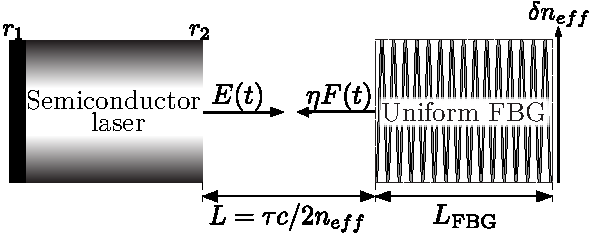
\includegraphics[width=\linewidth]{Images/FBG_setup_dneff_only_1col.pdf}
    \caption{Sketch of an optical fiber with an FBG written along its length.}
    \label{fig:FBG_setup}
\end{figure}
%
\par
%
An FBG is defined as a periodic modulation $\delta n_{eff}(z)$ of the refractive index with period $\Lambda$ along an optical fibre of length $L_\text{FBG}$.
The number of gratings in an FBG is therefore $N = L_\text{FBG}/\Lambda$. The most general form of this periodic modulation is
%
\begin{equation}
\label{eq:dneff}
    \delta n_{eff}(z) = \dnbar(z) \left[ 1 + v \cos{\left( \frac{2 \pi}{\Lambda} z + \phi(z) \right)} \right].
\end{equation}
%
Here, $\dnbar(z)$ describes the envelope of the periodic modulation along $L_\text{FBG}$; for example, $\dnbar(z) \sim e^{-z^2}$ yields a Gaussian refractive index profile. 
In addition to the envelope, $v$ denotes the fringe visibility of the index modulation, and $\phi(z)$ allows variation of the grating period along the fibre, enabling different frequencies to be reflected at different positions.
This flexibility allows tailoring of the spectral response through modulation depth and phase, directly influencing the accessible ECM structure.
%
\par
%
Light propagating in the fibre and interacting with the FBG undergoes diffraction when its wavelength is close to the design wavelength, $\lambda_D = 2 n_{eff} \Lambda$.
It is typically assumed that the light undergoes only first-order diffraction, which dominates in FBGs, so that a single propagating mode need be considered.
In this case, using coupled-mode theory and the synchronous approximation, one can derive coupled first-order differential equations describing the interaction between the forward- and backward-propagating waves, $R(z)$ and $S(z)$, respectively.
%
\begin{equation}
\label{eq:wave_eqs}
    \begin{aligned}
        \frac{dR}{dz} &= i \hat{\sigma} R(z) + i \k S(z) \\
        -\frac{dS}{dz} &= i \hat{\sigma} S(z) + i \k R(z)
    \end{aligned}
\end{equation}
%
with $R(z) = A(z) \exp{ \left( -i \left( \phi/2 -\delta z \right) \right) }, \; S(z) = B(z) \exp{ \left( -i \left( \phi/2 + \delta z \right) \right) }$.
For further details, see \cite{erdogan1997fiber} and references therein.
The parameters $\delta$, the wavevector mismatch, $\kappa$, the alternating-current (AC) coupling coefficient, and $\hat{\sigma}$, the direct-current (DC) self-coupling coefficient, are given by
%
\begin{align}
    \label{eq:delta}
    \delta &= 2 \pi \neff \left( \frac{1}{\lambda} - \frac{1}{\lambda_D} \right) \\
    \label{eq:kappa}
    \k &= \frac{\pi}{\lambda} v \dnbar(z)\\
    \label{eq:sigma}
    \hat{\sigma} &= \frac{2\k}{v} + \delta -\frac{1}{2}\frac{d\phi}{dz}.
\end{align}
%
Since $\k$ and $\hat{\sigma}$ may depend on $z$, \eqref{eq:wave_eqs} cannot in general be solved analytically, but they can be readily solved numerically once $\Lambda$, $n_{eff}$, $\dnbar(z)$, $\phi(z)$, and $L_\text{FBG}$ are specified.
%
\par
%
At this point, all the necessary ingredients are in place to calculate the key characteristic of an FBG, its reflection spectrum $\rho(\w)$.
Physically, the primary interest lies in the reflection spectrum of light reflected at the front FBG interface, assuming no reflection from the back interface.
Therefore, \eqref{eq:wave_eqs} is typically solved by setting $z = 0$ at the midpoint of the FBG, imposing boundary conditions $R(-L_\text{FBG}/2) = 1$ and $S(L_\text{FBG}/2) = 0$, and integrating backwards from $L_\text{FBG}/2$ to $-L_\text{FBG}/2$. The amplitude reflection coefficient is then given by
%
\begin{equation}
\label{eq:rho}
    \rho_\text{FBG} = \frac{S(-L_\text{FBG}/2)}{R(-L_\text{FBG}/2)}
\end{equation}
%
which defines the reflection spectrum $\rho(\w)$.
Although \eqref{eq:wave_eqs} must generally be solved numerically and closed-form expressions for $\rho(\w)$ are rarely available, certain standard grating designs such as uniform or raised-cosine-apodised gratings admit analytic solutions and provide valuable insight into the typical properties of FBG reflection spectra.
Among the different grating profiles, the simplest and most widely studied is the uniform grating.
%
%
\subsubsection*{Uniform FBG reflection spectra}
\label{subsubsec:FBG_feedback}
%
The uniform FBG is the canonical case, characterised by a constant grating period and uniform modulation depth.
Beyond being analytically tractable, it is also widely fabricated, providing a baseline for more advanced apodised or chirped gratings and a useful reference for understanding how FBG feedback influences ECM control.
For uniform gratings, the grating chirp satisfies $\sfrac{d\phi}{dz} = 0$ and the apodisation $\dnbar = \text{const.}$, so that the grating index variation given by \eqref{eq:dneff} reduces to a sine wave, as shown in Figure~\ref{fig:FBG_setup}.
Therefore, $\k$ and $\hat{\sigma}$ are constant in $z$, which allows the reflection spectrum $\rho(\w)$ to be obtained analytically by solving \eqref{eq:wave_eqs} and then evaluating \eqref{eq:rho}.
%
\begin{equation}
\label{eq:uniform_rho}
    \rho = \frac{-\k \sinh\left( L_\text{FBG}\right)}{\hat{\sigma} \sinh\left(\gamma L_\text{FBG}\right) + i\gamma \cosh\left(\gamma L_\text{FBG}\right)}
\end{equation}
%
where $\gamma = \sqrt{\k^2 - \hat{\sigma}^2}$ determines whether the field decays or oscillates within the grating. 
Several key features of the reflection spectrum $\rho(\w)$ are most clearly visualised by plotting it as a function of normalised frequency detuning while varying $\kappa L_\text{FBG}$ for a fixed $N$ \cite{erdogan1997fiber}.
%
\begin{equation*}
    \frac{\w - \w_\text{max}}{\w_\text{max}} = \frac{\hat{\sigma} L_\text{FBG}  }{\pi N}
\end{equation*}
%
Figure~\ref{fig:uniform_spectra_varykL} shows representative amplitude reflectivity and group delay spectra for three uniform gratings, plotted against normalised frequency detuning. 
The gratings are centred at the common laser wavelength of 1550 nm, with $\kappa L_\text{FBG} \in {0.5, 2, 5}$ and a fixed $N = 5000$, chosen to illustrate weak, moderate, and strong coupling regimes.
Increasing $N$ (and thus $L_\text{FBG}$) results in a narrower reflection bandwidth, whereas decreasing $N$ (and thus $L_\text{FBG}$) produces a broader one, provided that $\kappa L_\text{FBG}$ remains constant.
The reflection spectrum consists of a main lobe and a series of side lobes, separated by reflection zeros that are symmetrically spaced in wavelength on either side of the main lobe.
For gratings with low $\kappa L_\text{FBG}$, such as 0.5, the main lobe has a bandwidth, defined as the interval between its reflection zeros, that is twice the width of the side lobes \cite{erdogan1997fiber}.
Evidently, increasing $\kappa L_\text{FBG}$ increases the grating's maximum reflectivity and also broadens the main-lobe bandwidth while narrowing that of the side lobes.
Additionally, the time delay is approximately constant for low reflectivities but becomes increasingly distorted as $\kappa L_\text{FBG}$ increases.
Away from the main lobes, the time delays across all three cases are approximately the same, due to keeping the number of grating periods $N$ constant.
%
\begin{figure}[!t]
    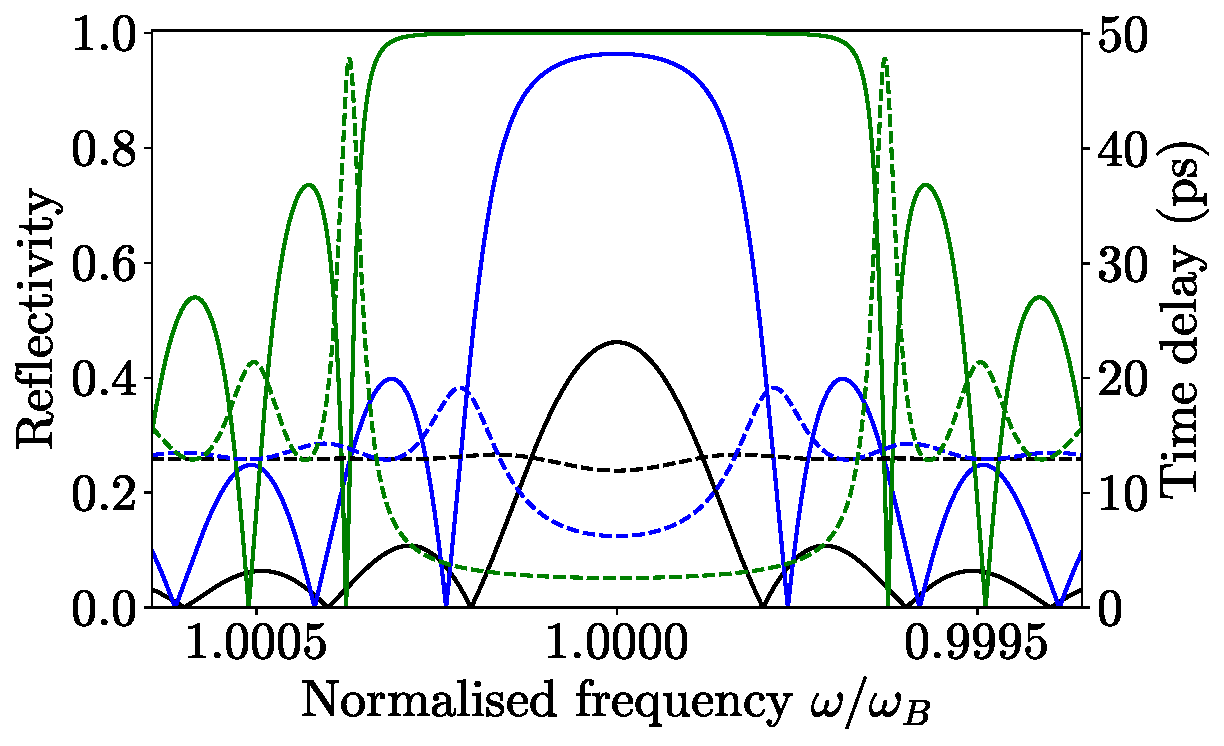
\includegraphics[width=\linewidth]{Images/Uniform_varying_kL_Rtau.pdf}
    \caption{Examples of aplitude reflectivity and group delay of uniform FBG reflection spectra with varying dimensionless grating strength $\k L_\text{FBG} \in [0.5, 2, 5]$ and constant number of grating periods $N=5000$.}
    \label{fig:uniform_spectra_varykL}
\end{figure}
%
\par
%
While varying $\kappa L_\text{FBG}$ suffices to illustrate the dependence on coupling strength without further substitutions, exploring changes in $\dnbar$ or $L_\text{FBG}$ requires expressing the frequency dependence explicitly.
Since $\kappa$ and $\hat{\sigma}$ depend only on wavelength and the prescribed grating parameters, the reflected amplitude $|\rho(\w)|$ and time delay can be directly plotted against frequency by substituting \eqref{eq:kappa} and \eqref{eq:sigma} into \eqref{eq:uniform_rho}.
Figure~\ref{fig:uniform_spectra_varyLdneff} shows examples of reflection spectra of uniform FBGs plotted against frequency, with the design frequency given by
%
\begin{equation}
    \w_D = \frac{\pi c}{\Lambda n_{eff}^2}
\end{equation}
%
highlighted to demonstrate the intrinsic shift of the Bragg resonance from the design frequency. The reflection spectrum of a uniform grating has a maximum reflectivity
%
\begin{equation}
\label{eq:rmax}
    R \equiv |\rho_\text{max}| = \tanh{(\k L_\text{FBG})}
\end{equation}
%
centred at the Bragg frequency $\w_\text{max}$,
%
\begin{equation}
\label{eq:wBragg}
    \w_\text{max} = \frac{\w_D}{\left( 1 + \frac{\dnbar }{\neff}\right)}
\end{equation}
%
corresponding to the peak reflectivity.
We note that $R$ is more commonly used to denote reflected power rather than reflected amplitude; however, the present notation is adopted for clarity in later sections.
The first zeros on either side of the main lobe occur at $\w_\text{max} \pm \w_z$, where
%
\begin{equation}
\label{eq:wz}
    \w_z = \w_\text{max} \sqrt{\left( \frac{\dnbar}{2 \neff} \right)^2 + \frac{1}{N^2} }
\end{equation}
%
and the phase of the reflection spectrum shifts by $2\pi$ between these zeros.
Outside the main lobe, the reflectivity peaks of the side lobes decay exponentially, with a $\pi$ phase change across each sidelobe.
%
\begin{figure}[!t]
    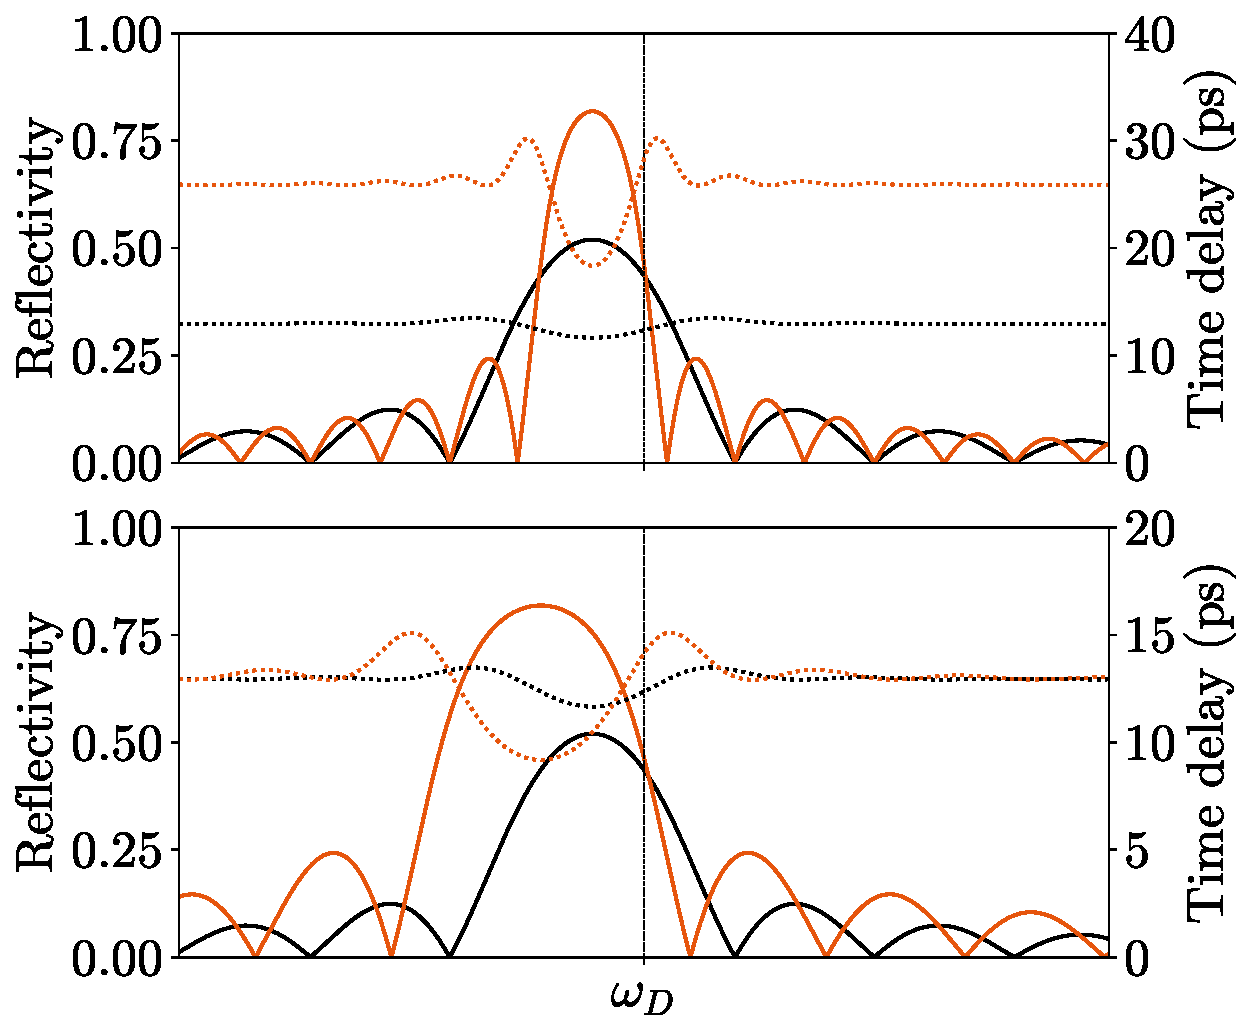
\includegraphics[width=\linewidth]{Images/Uniform_varying_L_dneff.pdf}
    \caption{Examples of the magnitude and group delay of uniform FBG reflection spectra, illustrating the effect of varying $\dnbar$ and $L_\text{FBG}$. 
    The nominal case (black curves) corresponds to $\dnbar = 5\e{-5}\neff$ and $L_\text{FBG} = 2.64,\text{mm}$; in (a) the grating length is doubled to $L_\text{FBG} = 5.28,\text{mm}$, and in (b) the index change is doubled to $\dnbar = 1\e{-4}\neff$.}
    \label{fig:uniform_spectra_varyLdneff}
\end{figure}
%
\par
%
Figure~\ref{fig:uniform_spectra_varyLdneff}(a) shows that doubling $L_\text{FBG}$ increases $R$ because more grating periods contribute to reflection, reducing transmission. 
At the same time, the bandwidth of each lobe is halved, while the shift of the reflection maximum from the design frequency remains unchanged. 
In addition, the group delay is approximately doubled, since the light interacts with twice as many grating periods.
In contrast, doubling $\dnbar$, as shown in (b), again increases $R$, but now the shift from the Bragg resonance increases while the bandwidth remains unchanged. 
The time delay is approximately the same between both cases, since the number of grating periods is unchanged.
Because these two parameters jointly determine the three key spectral features (resonance shift, maximum reflectivity, and bandwidth), it is not possible to vary one feature independently of the others.
Instead, a slight compensation to the grating period $\Lambda$ can be made, which shifts $\w_\text{max}$ while leaving $\wz$ and $R$ essentially unchanged.
This holds because laser centre frequencies are in the THz range, whereas the frequency offset is at most in GHz, so $\w_\text{max}/\w_D = \Lambda_D/\Lambda_\text{max} \approx 1$.
Using this approximation, together with \eqref{eq:wBragg} and \eqref{eq:wz}, $\dnbar$, $L_\text{FBG}$, and $\Lambda$ can be calculated sequentially using
%
\begin{align}
\label{eq:spec2phys}
    \dnbar &\approx \frac{2\wz}{\w_\text{max}} \frac{\neff}{\sqrt{1 + \left(\frac{\pi}{\arctanh{(R)}} \right)^2}},
    \\
    \Lambda &= \frac{\pi c}{\w_\text{max} \neff (\neff +\dnbar)},
    \\
    L &= \frac{\Lambda}{\sqrt{\left( \frac{\wz}{\w_\text{max}} \right)^2 - \left( \frac{\dnbar}{2\neff} \right)^2}}.
\end{align}
%
These expressions provide a direct inversion from spectral targets (bandwidth, reflectivity, and centre frequency) to physical grating parameters, enabling practical FBG design from desired optical specifications.
Taken together, these analytic results for uniform gratings provide the essential foundation for incorporating FBGs into feedback models of semiconductor lasers. 
This framework links grating design directly to ECM structure and dynamics, setting the stage for analysing FBG feedback within the LK equations.
%
%
\section*{FBG distributed feedback}
\label{sec:FBG_feedback}
%
The spectral selectivity of FBGs, combined with their practical advantages already noted such as all-fibre integration, low insertion loss, and design flexibility, makes them especially well suited for FOF in semiconductor laser systems. 
Building on the analytic understanding of uniform gratings, FBGs provide a direct route to reshaping the ECM structure in semiconductor lasers by tailoring their feedback spectrum. 
This dual role, as practical devices and theoretical benchmarks, has motivated investigations of how FBG feedback modifies semiconductor laser dynamics within the LK framework.
A schematic of a semiconductor laser under external feedback from an FBG is shown in Figure~\ref{fig:FBG_setup}.
As discussed in \ref{subsubsec:FBG}, the reflection spectrum of an FBG can exhibit considerable complexity. 
Since an FBG acts as a spectral filter, the feedback term $F(t)$ is given by \eqref{eq:FOF} with reflection spectrum $\rho(\w)$ given by \eqref{eq:uniform_rho}.
Equivalently, the feedback term can be expressed as a time-domain convolution,
%
\begin{equation}
    \label{eq:convolution}
     F(t) = e^{-i C_p} \tilde{\rho}(t) \otimes E(t-\tau)
\end{equation}
%
where $\tilde{\rho}(t)$ denotes the impulse response of the FBG relative to the Bragg resonance frequency.
Analytic expressions typically do not exist for the impulse response, even for simple gratings, and are therefore usually calculated numerically through fast Fourier transforms (FFTs), for example.
The need to compute $F(t)$ numerically restricts analysis to direct integration of the solutions $(E(t),N(t))$ and subsequent evaluation of time-series properties such as maximal Lyapunov exponents (MLEs) or spectral measures such as signal dispersion.
In contrast to the Lorentzian FOF case, no analytic reduction to a discrete DDE system has been proposed, making FBG feedback intrinsically more difficult to analyse.
Despite the substantial computational and analytical challenges posed by this feedback term, several studies have investigated uniform FBG feedback using the convolution representation for $F(t)$ given by \eqref{eq:convolution} \cite{li2012distributed, li2015chaotic, li2020stable, jiang2021characterizing, skenderas2021feedback, skenderas2024impact}.
%
\par
%
Early studies of FBG feedback relied mainly on numerical investigations, which provided limited analytic insight but revealed several important features of the resulting dynamics. 
A primary motivation was the generation of broadband chaotic signals for applications such as high-speed optical random bit generation \cite{uchida2008fast} and chaos-based secure communication \cite{annovazzi2008secure}. 
Compared with conventional mirror feedback, FBG feedback was shown to suppress the time-delay signature (TDS) much more effectively, thereby concealing the EC delay that autocorrelation-based attacks can exploit in encryption systems \cite{li2012distributed, jiang2021characterizing}. 
This improvement was attributed to the distributed reflections along the FBG, which spread out the effective feedback delay. 
Numerical studies demonstrated that TDS suppression improves as the FBG bandwidth decreases, owing to the stronger group-delay dispersion introduced by narrower gratings, while the FBG length plays little role in the suppression \cite{li2012distributed}. 
However, this benefit comes with a trade-off: as the bandwidth narrows, the parameter regions supporting chaos shrink and are progressively replaced by stable period-1 oscillations \cite{li2020stable}. 
Interestingly, FBG feedback can also generate chaos at shorter delays than mirror feedback, broadening the design space for compact devices \cite{li2012distributed}. 
Beyond bandwidth effects, detuning between the laser frequency and the Bragg frequency plays a critical role: optimal TDS suppression occurs under positive detuning, consistent with the red-shift of the cavity resonance induced by the antiguidance effect \cite{li2015chaotic}. 
Together, these results established FBG feedback as both a practical route to more secure chaotic carriers and a rich platform for exploring how spectral filtering reshapes external feedback laser dynamics.
%
\par
%
The convolution representation for $F(t)$ can also be expressed as a distributed delay term. 
By definition,
\begin{equation*}
\tilde{\rho}(t) \otimes E(t-\tau) = \int_{-\infty}^{\infty} \tilde{\rho}(t-s) E(s-\tau)\,ds.
\end{equation*}
%
To render the integral finite, note first that $E(s-\tau) = 0$ for $s > t+\tau$, while the lower bound can be truncated at $t-T$, with $T$ chosen such that $\tilde{\rho}(s) \approx 0$ for all $s > T$, yielding an expression for $F(t)$ suitable for numerical integration
%
\begin{equation}
    \label{eq:distributed}
F(t) \approx e^{-i C_p} \int_{t-T}^{t+\tau} \tilde{\rho}(t-s) E(s-\tau)\,ds.
\end{equation}
%
This integral form highlights that FBG feedback acts as a weighted superposition of past fields, directly reflecting the spectral filtering imposed by the grating and contrasting with the single discrete delay characteristic of conventional optical feedback.
Both representations for $F(t)$ in \eqref{eq:convolution} and \eqref{eq:distributed} introduce numerical inaccuracies: truncation of the impulse response $\tilde{\rho}(t)$ limits the effective memory of the feedback, while discretisation of $\tilde{\rho}(t)$ or its frequency counterpart $\rho(\w)$ introduces sampling errors.
Such errors accumulate in the computation of the convolution or distributed-delay integral, setting practical limits on the accuracy of FBG feedback simulations.
%
\par
%
Motivated by the need for stronger dispersion to enhance TDS suppression, this distributed-delay formulation has also been applied to chirped fibre Bragg gratings (CFBGs) \cite{wang2017time, wang2019key, wang2023critical, chao2020permutation}.
Because analytic reflectivity spectra are unavailable for chirped gratings, \eqref{eq:wave_eqs} must be solved numerically, further increasing computational cost.
As in the uniform case, the impulse response $\tilde{\rho}(t)$ is obtained via FFTs and incorporated into the delay term.
Numerical studies demonstrated that CFBG feedback suppresses the TDS more effectively than uniform gratings and, in some cases, eliminates it entirely without requiring additional amplification, thereby simplifying experimental configurations.
In addition, the broader dispersion of CFBGs enriches the dynamical behaviour of the laser and expands the parameter space accessible for chaos-based applications, highlighting both the promise and the added complexity of chirped grating feedback compared to uniform designs.
%
\par
%
More recently, investigations have extended beyond the generation of chaotic signals, yet, as in earlier work, the use of the convolution representation for $F(t)$ has confined most studies to numerical integration of time series. 
\Skenderas \textit{et al.} carried out a series of studies examining how detailed spectral features of FBGs impact semiconductor laser stability \cite{skenderas2021feedback, skenderas2022influence, skenderas2024impact}. 
They showed that the positions of the zeros in the FBG reflection spectrum exert a strong influence on stability, with fluctuations emerging when these zeros overlap with the relaxation oscillation side lobes of the laser. 
This effect was quantified by tracking the feedback rate required to trigger Hopf bifurcations for gratings of varying length (and thus bandwidth), highlighting that longer (narrower-band) gratings introduce stability oscillations even when overall reflectivity is kept constant. 
An important observation was that detuning asymmetry, long observed in FBG feedback, was confirmed to be an intrinsic feature of the interaction between the spectral phase of the grating and the laser dynamics. 
In later experimental work, they further demonstrated that small variations in the feedback phase, such as those induced by thermal tuning of the grating, can produce significant cyclic changes in stability, showing that both offset phase and phase fluctuations play a crucial role in shaping the dynamics \cite{skenderas2024impact}. 
Overall, these studies show that while FBG feedback shares many broad features with filtered optical feedback, the detailed shape of the reflection spectrum—its zeros, side lobes, and phase—adds layers of complexity that strongly affect stability boundaries. 
%
\par
%
While the convolution representation of $F(t)$ has provided limited insight into FBG feedback, no work has systematically analysed the external cavity mode (ECM) structure under FBG feedback, with the sole exception of studies by Naumenko \textit{et al.} \cite{naumenko2003characteristics,naumenko2004slow}
Their approach uniquely extended the analysis into the strong-feedback regime by adopting a multiple-reflection model, originally proposed for plain mirrors, and adapting it to the case of FBGs.
In this framework, the feedback term $\eta e^{-i C_p}E(t-\tau)$ in the LK equations is replaced by $E(t)\ln[E_r(t)/E(t)]$, where $E_r(t)$ represents the infinite series of external cavity reflections.
This reduces to the usual single-reflection term in the weak-feedback limit, but crucially retains the higher-order contributions required to capture the altered ECM structure when strong, frequency-selective feedback is present.
Here, the spectral filtering of the FBG enters explicitly through $\rho(\w)$, enabling the use of a Green-function formalism to derive stationary ECM conditions.
This provided, for the first time, a direct connection between the reflection spectrum of FBGs and the organisation of ECMs.
%
\par
%
Their results showed that, under weak feedback, ECMs remain largely confined to the main lobe of the FBG reflectivity, with the maximal gain mode (MGM) shifted close to the Bragg resonance frequency, reproducing the scenario found earlier for Lorentzian FOF.
As the FBG bandwidth narrows, however, new “satellite” ECM branches emerge, separated from the main ECM ellipse by the reflection zeros of the grating.
Under strong feedback, these satellites evolve into additional families of modes located within the side lobes of the FBG spectrum, fundamentally altering the accessible mode structure.
Follow-up investigations deepened these insights by examining dynamical consequences: the reshaped ECM structure could either suppress or destabilise low-frequency fluctuations depending on grating bandwidth and reflectivity, while intensity-noise studies revealed that strong FBG filtering not only generates new steady-state branches but also reshapes the balance between stable modes and antimodes.
%
\par
%
Together, these works demonstrate that an ECM-focused analytical treatment, rather than purely convolution-based time series simulation, provides unique insight into how FBG feedback reshapes both the topology and stability of the mode structure.
Yet, the complexity of the feedback term meant that full bifurcation analysis was not achieved, and these studies remain the only systematic attempt to connect the spectral features of FBGs—zeros, bandwidth, and side lobes—directly to the mode structure and noise properties of semiconductor lasers.
At the same time, the approach is computationally demanding: calculating ECMs requires solving intricate mode equations from the multiple-reflection expansion, while numerical integration is limited by both accuracy issues and long runtimes.
In addition, the formulation does not readily support advanced bifurcation tools such as numerical continuation, leaving the global organisation of solutions only partially characterised.
%
\par
%
Taken together, this review highlights the need for a modelling framework that unifies analytic tractability and numerical efficiency, something not achieved by current treatments of FBG feedback.
Ideally, such a model would preserve the physical accuracy of FBG feedback, yet remain mathematically tractable, yielding closed-form ECM conditions and enabling stability analysis available to existing filtered-feedback models.
At the same time, it should support efficient and accurate numerical integration, free from the heavy computational costs and accuracy concerns that currently constrain the current integro-differental equation formulations.
Developing such a framework would not only unify the fragmented perspectives on FBG feedback but also provide a practical tool for connecting grating design to laser dynamics in a transparent and predictive way.


% --- Summary of Introduction ---
% Semiconductor lasers are central to modern photonic technology, particularly in optical communications where their emission wavelengths align with network standards. Beyond their technological role, they also serve as paradigmatic systems for exploring nonlinear dynamics, since feedback turns their governing equations into delay differential equations (DDEs) with broad relevance across physics, engineering, and biology.
% External optical feedback (EOF) strongly shapes laser behaviour. The seminal Lang–Kobayashi (LK) equations first captured this by modelling a single-mode semiconductor laser under conventional optical feedback (COF) from a mirror. These equations revealed how external cavity modes (ECMs) emerge and interact, and their DDE structure allowed powerful analytical tools and numerical continuation to be applied. Since then, alternative feedback schemes have been explored. Phase-conjugate feedback (PCF) introduces symmetry that reorganises ECMs into isolated branches, while filtered optical feedback (FOF), especially with Lorentzian filters, has been studied in depth thanks to its analytic tractability. These studies showed that filtering reduces the number of ECMs, stabilises dynamics, and produces rich bifurcation structures, including codimension-2 and codimension-3 points that organise transitions in mode structure.
% Within this landscape, fibre Bragg gratings (FBGs) have attracted intense interest. They are all-fibre, low-loss, low-cost components whose reflectivity spectra can be precisely engineered. Uniform FBGs provide analytic solutions that serve as benchmarks, clarifying how reflectivity, bandwidth, and resonance shift depend on physical parameters. More advanced chirped FBGs (CFBGs) offer stronger dispersion and improved suppression of time-delay signatures (TDS), which is crucial for chaos-based communications. However, modelling feedback from FBGs poses challenges. Convolution- and distributed-delay formulations allow numerical time-series simulation but give only limited dynamical insight. Analyses of stability have shown roles for reflection zeros and detuning, but the mode structure itself has resisted systematic study.
% The one major exception is a series of works that extended ECM analysis to FBG feedback using a multiple-reflection framework. These studies demonstrated that spectral features of FBGs—zeros, side lobes, and bandwidth—directly reshape the ECM structure, creating new families of modes and altering noise properties. Yet this approach is computationally heavy, difficult to extend with bifurcation tools, and limited in scope.
% This review therefore highlights a critical gap: while existing models either enable analytic tractability (mirror and Lorentzian FOF) or capture physical realism (FBGs via convolution), no framework yet combines both. The field remains without a transparent, computationally efficient, and predictive model that can connect FBG design directly to laser dynamics while retaining compatibility with powerful DDE analysis tools.